\chapter{General Discussion \& Conclusion}
% We did good
We used a case study of the impact of climate change on the joint provision of forest ecosystem services to demonstrate the utility of a new measure of pairwise objective conflict and to demonstrate a new application of existing conflict measures in the quantification of conflict within and among multi-objective systems.

% We did good in something that was hard to do good in
We argue that this case study served as a rigorous first test of the conflict measures and conflict quantification process, because there was little overall conflict in these systems and the differences in relative objective achievement across climate scenarios were not great. For instance, in the case study, the hypervolume indicator for each climate scenario was relatively large, with solutions occupying over 80\% of the objective space in all cases. In addition, in all but one pairwise objective comparison, it was difficult to discern any distinct conflict relationship between the objectives. As a result, our proposed conflict metric and the hypervolume indicators were required to detect subtle differences in conflict, which we claim they did adequately. Should the differences in objective achievement between climate scenarios have been more pronounced, or should the objectives have been in greater conflict with one another, we suspect the utility of these measures and the process we demonstrated here would only increase.

For comparison, we cite the DTLZ 1 and DTLZ 2 reference problems \cite{deb2002scalable}. Their frontiers are shown in Figure \ref{fig:dtlzFrontiers} (note that the objectives are minimized). The hypervolume indicator for DTLZ 1 is 0.4995, and the hypervolume indicator for DTLZ 2 is 0.2140. Conflict metrics for the objectives are 0.574 and 0.707 for DTLZ 1 and DTLZ 2, respectively. We provide this information simply to indicate the ability of our conflict quantification process to respond to larger differences in the Pareto frontiers. That is, when relationships among the objectives vary substantially, so too do the hypervolume indicator and conflict metric.

\begin{figure}[ht]
\centering
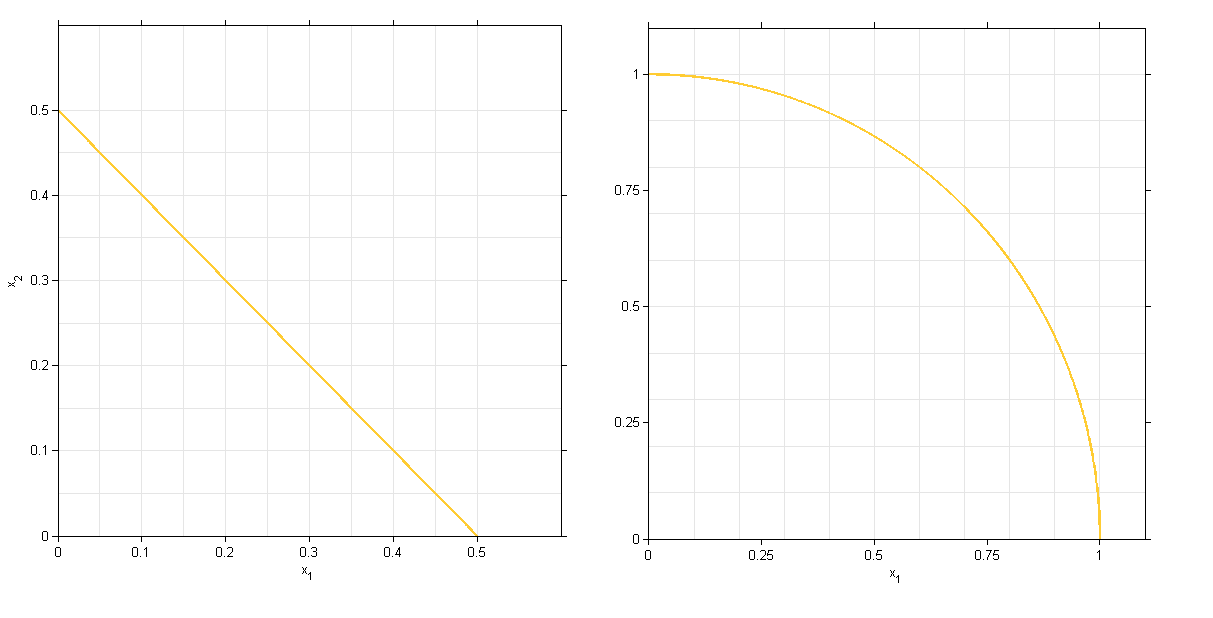
\includegraphics[width=.9\textwidth]{../images/DTLZFrontiers_1and2}
\caption[Frontiers of the DTLZ 1 and DTLZ 2 test problems]{Frontiers for the DTLZ 1 and DTLZ 2 test problems. All objectives are minimized. The hypervolume indicator for DTLZ 1 is 0.4995, and the hypervolume indicator for DTLZ 2 is 0.2140. Conflict metrics for the objectives are 0.574 and 0.707 for DTLZ 1 and DTLZ 2, respectively.}
\label{fig:dtlzFrontiers}
\end{figure}

% But who's to say that it will always do good. It may not. You'd want to also consider other scenarios, like this food processing one
Of course, our apparent success in quantifying and differentiating conflict in this case study does not guarantee similar results in other studies. In consideration of different climate change scenarios, different ecosystem services, or a different study area, the conflict measures may prove less insightful. Further tests are needed in other multi-objective systems as well, such as hospitals, aircraft design, and other applications beyond natural resource management.

Let us consider again the manager of the food processing facility, and imagine they are trying to determine in which country to open an additional facility. Each country has a different regulation on the allowable level of microbiological content. The manager could run their multi-objective study under each of these various regulatory regimes and use the hypervolume indicator to determine how conflict between nutrient content and processing time changes. Armed with this knowledge, they may decide on the location of their new facility based on the extent of that conflict. For instance, if one of the proposed new locations offers greater joint provision of the objectives (a larger hypervolume), then the manager has at their disposal a set of alternatives which is arguably better because the required relative sacrifices are less. This is attractive and may help determine that this is the location they should select.

Or consider a decision maker working for an agency which distributes funding to hospitals. The hospitals have all undergone a multi-objective study comparing operating costs to expected loss of life. Obviously, the hospital seeks to minimize both of these objectives. The decision maker at the funding agency may use the pairwise conflict metric introduced in section \ref{sec:newConflictMetric} to determine for which hospitals the conflict between these objectives is strongest. They may wish to provide financial assistance to those hospitals which suffer from the most conflict.

%As a final example, we use the Drink Area case study presented in Chapter \ref{ch:caseStudyDeschutes}. We saw that the fire hazard under the climate scenarios is predicted to increase. Aware of this, the USFS may decide to implement additional or more intensive fuel removal actions. However, the consequences in terms of sediment delivery are predicted to increase as well, meaning that the watershed will contain a higher sediment content than before. If this trend continues and sediment levels pass some specified threshold, the USFS may deem it necessary to install a filtration system.

% We think our thing would continue to do good, bc, again, it did good here. It was so great. Bigly.
Based on the results presented here, we believe that our new conflict measure and the process we suggest would be useful to the managers in these cases as well. As we saw in the case study, the proposed conflict measure was successful in being able to identify which objective pairs were most in conflict. We also saw that the hypervolumes were successful in detecting increasing system conflict under different environmental conditions. These variations in conflict were supported by the underlying model data. 

% But it's not perfec
However, the new conflict metric and process are not without shortcomings. We first note that $C_{ij}$ is susceptible to relatively large variations in cases where neither the distance component $c_{ij,d}$ nor the rank correlation component $c_{ij,\rho}$ tend toward their $[0,1]$ bounds. In these cases, the components have more influence on the value of the conflict metric $C_{ij}$, so slight variations can lead to relatively large differences. In addition, differences in system conflict cannot be totally explained by the collection of pairwise conflict measures. For instance, while the small pairwise conflict metrics in the case study ($< 0.4$) coarsely correspond to large hypervolumes ($> 0.8$), we cannot use them to explain the source of the small differences observed in hypervolume. In fact, for the climate scenario with the most system conflict, E85, the sum of its pairwise conflict metrics was smallest. Lastly, the conflict measures used in the proposed process can be difficult to interpret, since they provide results in terms of relative objective achievement. That is, instead of having results that are measurable in the dimensions of the objectives, they are in percent achievements for the objectives.

% So we need to do more research, more case studies, and we need to try to make our tool better. But all in all, we're awesome. Over and out.
In summary, we have provided a foundation for quantitative conflict analysis for the comparison of multi-objective systems. Our results show that our proposed process and the new pairwise objective conflict metric are successful in quantifying and differentiating the amount of conflict within and across multi-objective systems and that they stand to serve as a useful tool for multi-objective decision making. However, more experimentation with this conflict analysis is required to better understand the limitations of its utility, and refinements to the new pairwise conflict measure should be investigated. Especially useful refinements would be those which address the variation in the conflict metric when neither of its components tends towards a limiting value of 0 or 1.